\documentclass{article}\usepackage[]{graphicx}\usepackage[]{xcolor}
% maxwidth is the original width if it is less than linewidth
% otherwise use linewidth (to make sure the graphics do not exceed the margin)
\makeatletter
\def\maxwidth{ %
  \ifdim\Gin@nat@width>\linewidth
    \linewidth
  \else
    \Gin@nat@width
  \fi
}
\makeatother

\definecolor{fgcolor}{rgb}{0.345, 0.345, 0.345}
\newcommand{\hlnum}[1]{\textcolor[rgb]{0.686,0.059,0.569}{#1}}%
\newcommand{\hlsng}[1]{\textcolor[rgb]{0.192,0.494,0.8}{#1}}%
\newcommand{\hlcom}[1]{\textcolor[rgb]{0.678,0.584,0.686}{\textit{#1}}}%
\newcommand{\hlopt}[1]{\textcolor[rgb]{0,0,0}{#1}}%
\newcommand{\hldef}[1]{\textcolor[rgb]{0.345,0.345,0.345}{#1}}%
\newcommand{\hlkwa}[1]{\textcolor[rgb]{0.161,0.373,0.58}{\textbf{#1}}}%
\newcommand{\hlkwb}[1]{\textcolor[rgb]{0.69,0.353,0.396}{#1}}%
\newcommand{\hlkwc}[1]{\textcolor[rgb]{0.333,0.667,0.333}{#1}}%
\newcommand{\hlkwd}[1]{\textcolor[rgb]{0.737,0.353,0.396}{\textbf{#1}}}%
\let\hlipl\hlkwb

\usepackage{framed}
\makeatletter
\newenvironment{kframe}{%
 \def\at@end@of@kframe{}%
 \ifinner\ifhmode%
  \def\at@end@of@kframe{\end{minipage}}%
  \begin{minipage}{\columnwidth}%
 \fi\fi%
 \def\FrameCommand##1{\hskip\@totalleftmargin \hskip-\fboxsep
 \colorbox{shadecolor}{##1}\hskip-\fboxsep
     % There is no \\@totalrightmargin, so:
     \hskip-\linewidth \hskip-\@totalleftmargin \hskip\columnwidth}%
 \MakeFramed {\advance\hsize-\width
   \@totalleftmargin\z@ \linewidth\hsize
   \@setminipage}}%
 {\par\unskip\endMakeFramed%
 \at@end@of@kframe}
\makeatother

\definecolor{shadecolor}{rgb}{.97, .97, .97}
\definecolor{messagecolor}{rgb}{0, 0, 0}
\definecolor{warningcolor}{rgb}{1, 0, 1}
\definecolor{errorcolor}{rgb}{1, 0, 0}
\newenvironment{knitrout}{}{} % an empty environment to be redefined in TeX

\usepackage{alltt}
\usepackage{amsmath} %This allows me to use the align functionality.
                     %If you find yourself trying to replicate
                     %something you found online, ensure you're
                     %loading the necessary packages!
\usepackage{amsfonts}%Math font
\usepackage{graphicx}%For including graphics
\usepackage{hyperref}%For Hyperlinks
\usepackage[shortlabels]{enumitem}% For enumerated lists with labels specified
                                  % We had to run tlmgr_install("enumitem") in R
\hypersetup{colorlinks = true,citecolor=black} %set citations to have black (not green) color
\usepackage{natbib}        %For the bibliography
\setlength{\bibsep}{0pt plus 0.3ex}
\bibliographystyle{apalike}%For the bibliography
\usepackage[margin=0.50in]{geometry}
\usepackage{float}
\usepackage{multicol}

%fix for figures
\usepackage{caption}
\newenvironment{Figure}
  {\par\medskip\noindent\minipage{\linewidth}}
  {\endminipage\par\medskip}
\IfFileExists{upquote.sty}{\usepackage{upquote}}{}
\begin{document}\raggedcolumns

\vspace{-1in}
\title{Lab 10 -- MATH 240 -- Computational Statistics}

\author{
  Henry Sun \\
  Colgate University  \\
  Department of Mathematics  \\
  {\tt hlsun@colgate.edu}
}

\date{4/8/25}

\maketitle

\begin{multicols}{2}
%\raggedcolumns % If your spacing gets messed up try uncommenting 
                % this line
\begin{abstract}
In this week's lab, we conducted statistical analysis on Gallup poll data. Gallup suggests that doubling the sampling size will halve the margin of error (MOE). We show that this is actually not the case, as the margin of error depends on both the sample size ($n$) and the population proportion ($p$).
\end{abstract}

\noindent \textbf{Keywords:} Simulations; resampling; Wilson Estimate; margin of error
\section{Introduction}
Gallup polls published a document called ``\textit{How Are Polls Conducted?}" that describes how Gallup selects people to include in its poll and other details. Near the end of the document, Gallup stated that: 
\begin{center}
\textit{``For example, with a sample size of 1,000 national adults (derived using careful random selection procedures), the results are highly likely to be accurate within a margin of error of $\pm 4$ percentage points.”}
\end{center}
\begin{center}
\textit{``If Gallup increases a poll sample size to 2,000, the results would then be accurate within $\pm 2\%$ of the underlying population value, a gain of two percentage points in terms of accuracy, but with a $100\%$ increase in the cost of conducting the survey."}
\end{center}
\indent Gallup provided the results of a February 3-16, 2025 poll of 1,004 adults aged 18+ living in all 50 U.S. states and the District of Columbia, revealing that $39\%$ of of respondents were satisfied with the position of the United States in the world today, compared to $59\%$ that were dissatisfied and $2\%$ with no opinion. For this poll, Gallup reported a $\pm 4\%$ margin of error (MOE). \\
\indent When providing the MOE, we are aiming to describe the variation in our sample using the sample proportion $\hat{p}$ as an estimate of $p$. We are basically asking how much we expect sample proportion $\hat{p}$ to differ from the population proportion $p$. In order to maintain a small MOE, we have to make sure that the sample size is large enough, and that the sample is representative of the population, which we will explore in this lab. \\
\indent It is convention in statistics to report a margin of error that provides $95\%$ confidence, meaning that if we were to conduct the poll repeatedly, the interval would contain the actual proportion $95\%$ of the time. \\ 
\indent In this lab, we first began by calculating the MOE by conducting a basic simulation using 10k polls, assuming that we know $p$, the population proportion. \\
\indent We then used resampling to obtain a sampling distribution for $\hat{p}$ and calculated the MOE. \\
\indent Finally, we varied $n$ and $p$, conducting a simulation using 10k polls for each combination of $n$ and $p$, seeing how the estimated MOE and Wilson MOE varied with $n$ and $p$. 

% Provide an overarching summary of what you're talking about. In this section, you introduce the idea to the reader, and your goal is to pull them in. What's the mystery you aim to solve?
% 
% You want to provide enough background to understand the context of the work. Specifically, what is the question you are addressing? If it applies, describe what information currently exists about this problem, including citations, and explain how the question you're answering complements this work.
% 
% Provide a roadmap of the structure of the paper. 

% \subsection{Intro Subsection}
% You might need/want to discuss the topics in subsections. Or, you may have multiple questions.

\section{Methods}
For this lab, we are working with data given by Gallup polls. The results data from the polls were generated by creating a data frame with the exact proportions given in the poll. In order to plot our graphs and create tables, we used \texttt{ggplot2} \citep{ggplot2} and \texttt{xtable} \citep{xtable}. \texttt{patchwork} \citep{patchwork} was used to combined plots together. 

\subsection{Basic Simulation}
For our basic simulation, we assumed that the true probability/population proportion, $p$, of someone being satisfied with the position of the United States today is $0.39$. We could then simulate 10k polls using \verb|rbinom()| using these conditions, also using the sample size given by the Gallup poll, $n=1004$. We then repeated another simulation using the same conditions, except we doubled the sample size. 

\subsection{Resampling}
In the previous section, we had made the assumption that the population proportion $p$ was exactly $0.39$. However, in nearly any other situations, we are never given the true population proportion, nor are we able to just magically double the sample the sample size. Instead, we can use resampling of the original Gallup survey and plot the sampling distribution of $\hat{p}$, the sample proportion, for $1000$ resamples. 
\subsection{Simulation over $n$ and $p$}
In order to show how both sample size ($n$) and the population proportion ($p$) affect MOE, we conducted as similar procedure in the ``Basic Simulation" Section, except we varied $n$ from $100$ to $3000$ in increments of $10$ and $p$ from $0.01$ to $0.99$ in increments of $0.01$, and calculated the estimated MOE for each case. We then summarized the results by creating a \verb|geom_raster()| plot, showing MOE as function of $n$ and $p$. 

\subsection{Actual Margin of Error}
When finding the actual margin of error, we used the Wilson margin of error formula, given as: 
\[
\text{MOE}_{\text{w}} = z_{1-\alpha/2} \times \frac{ \sqrt{ n\hat{p}(1-\hat{p}) + \frac{{z_{1-\alpha/2}}^2}{4} } }{ n + {z_{1-\alpha/2}}^2 }
.\]
Where $z_{\alpha/2}$ is the z-score at the $\alpha/2$th percentile. \\
\indent For our lab, $\alpha =0.05$. We repeated the same procedure highlighted above in ``Simulation over $n$ and $p$" and summarized the results by creating another \verb|geom_raster()| plot. 

\section{Results}
\subsection{Basic Simulation}
Figure \ref{plot1} shows the histogram and superimposed density of the sampling distribution for $p$ and sample sizes. The red lines denote the population proportion $p$. Both plots show an approximately Gaussian distribution, but the histogram with the larger sample size has considerably less variation, showing that a larger sample size will lead to convergence towards the true $p$. 
\begin{Figure}
\centering
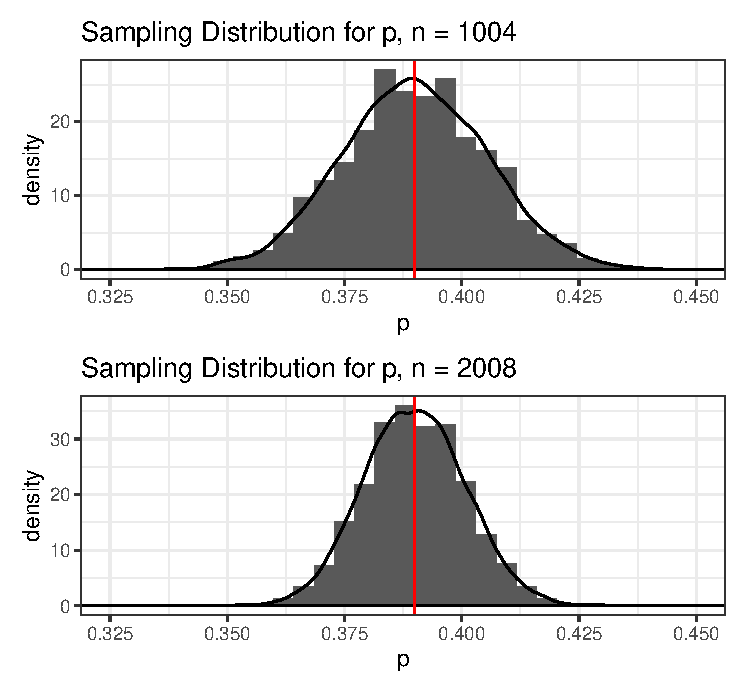
\includegraphics[width = 7cm, height = 6.15cm]{task1plots.pdf}
\captionof{figure}{Plots for the sampling distribution of $p$. The distribution is approximately Gaussian for both, but there is variation with $n = 2008$.} \label{plot1}
\end{Figure}

\begin{Figure}
% latex table generated in R 4.3.3 by xtable 1.8-4 package
% Tue Apr  1 07:26:31 2025
%\begin{table}[H]% YOU NEED TO REPLACE THIS WITH FIGURE
\centering
\begin{tabular}{lrrrr}
  \hline
n & Middle 95 & Estimated MOE & Gallup MOE \\ 
  \hline
1004 & 0.0608 & 0.0303 & 0.04 \\ 
  2008 & 0.0423 & 0.0211 & 0.02 \\ 
   \hline
\end{tabular}
%\caption{This is a table.} % YOU NEED TO CHANGE THIS TO captionof
\captionof{table}{Table comparing the estimated MOE compared to Gallup's reported MOE.} 
\label{table1}
%\end{table} % YOU NEED TO REPLACE THIS WITH FIGURE
\end{Figure}

As it turns out, Gallup's reported MOE for $n=1004$ is significantly off from the estimated MOE. For our lab, we calculated the estimated MOE by halving the range of the middle $95\%$, which is calculated by subtracting the $97.5$th percentile by the $2.5$th percentile. As we can see in the table (Table \ref{table1}), Gallup actually overestimated its MOE for the smaller sample size, although it's MOE for the larger sample size is roughly the same as the estimated MOE. In effect, we've showed that the original MOE of $4\%$ is not very precise, and that doubling the sample size will not halve the MOE.

\subsection{Resampling}
The figure (Figure \ref{plot3}) in the appendix shows this sampling distribution of $\hat{p}$, which is once again approximately Gaussian due to its large sample size, and centered around $0.39$, The estimated MOE calculating for this sampling distribution is $0.0304$, yielding similar results to the basic simulation MOE for the sample size. Once again, Gallup's reported MOE of $4\%$ is overestimating the estimated MOE from resampling. 

\subsection{Simulation of $n$ and $p$}
The figure below (Figure \ref{plot2}) show the \verb|geom_raster()| plots for both the estimated MOE (calculated by halving the middle $95\%$) and the Wilson MOE (calculated by the formula given before). In the top plot (the plot for the estimated MOE), we can see that the sample size is only one variable affecting the MOE. While sample size does reduce the MOE, MOE also changes with $p$. That is, when $p$ is extreme, the MOE is smaller. The intersection between the black line and the red line shows the estimated MOE at $n=1004$ and $p=0.39$, and the intersection between the black line and the red line shows the estimated MOE at $n=2008$ and $p=0.39$. We can clearly see that MOE decreases with a larger sample size, but not linearly. 
\subsection{Actual Margin of Error}
The bottom plot in figure \ref{plot2} shows pretty much the same thing highlighted in the \verb|geom_raster()| plot for the estimated MOE, except that we are calculating the actual Wilson MOE plotting it as a function of $n$ and $p$. This paints a nearly identical picture and yields similar results to the estimated MOE. The only noticeable difference is that the gradient between MOE boundaries are slightly smoother.

\section{Discussion}
As we've shown in this lab, the story isn't as simple as Gallup made it out to be. First of all, Gallup's estimates for the MOE were inaccurate to begin with. The estimated MOE for $n=1004$ is actually more like $3\%$ compared to Gallup's $4\%$. Gallup is actually \emph{overreporting} the MOE. However, Gallup's MOE and the estimated MOE are nearly identical when doubling the sample size. \\
\indent Although we did show in the basic simulations that doubling sampling size decreased the MOE, Gallup implies that doubling the sample size will correspond to halving the MOE. As shown above this is not true. Why? because MOE also depends on $p$, as shown by the \verb|geom_raster()| plots of the estimated MOE and the Wilson MOE. \\

%%%%%%%%%%%%%%%%%%%%%%%%%%%%%%%%%%%%%%%%%%%%%%%%%%%%%%%%%%%%%%%%%%%%%%%%%%%%%%%%
% Bibliography
%%%%%%%%%%%%%%%%%%%%%%%%%%%%%%%%%%%%%%%%%%%%%%%%%%%%%%%%%%%%%%%%%%%%%%%%%%%%%%%%
\vspace{2em}

\begin{tiny}
\bibliography{bib}
\end{tiny}
\end{multicols}

%%%%%%%%%%%%%%%%%%%%%%%%%%%%%%%%%%%%%%%%%%%%%%%%%%%%%%%%%%%%%%%%%%%%%%%%%%%%%%%%
% Appendix
%%%%%%%%%%%%%%%%%%%%%%%%%%%%%%%%%%%%%%%%%%%%%%%%%%%%%%%%%%%%%%%%%%%%%%%%%%%%%%%%
\newpage
\onecolumn
\section{Appendix}

\begin{Figure}
\centering
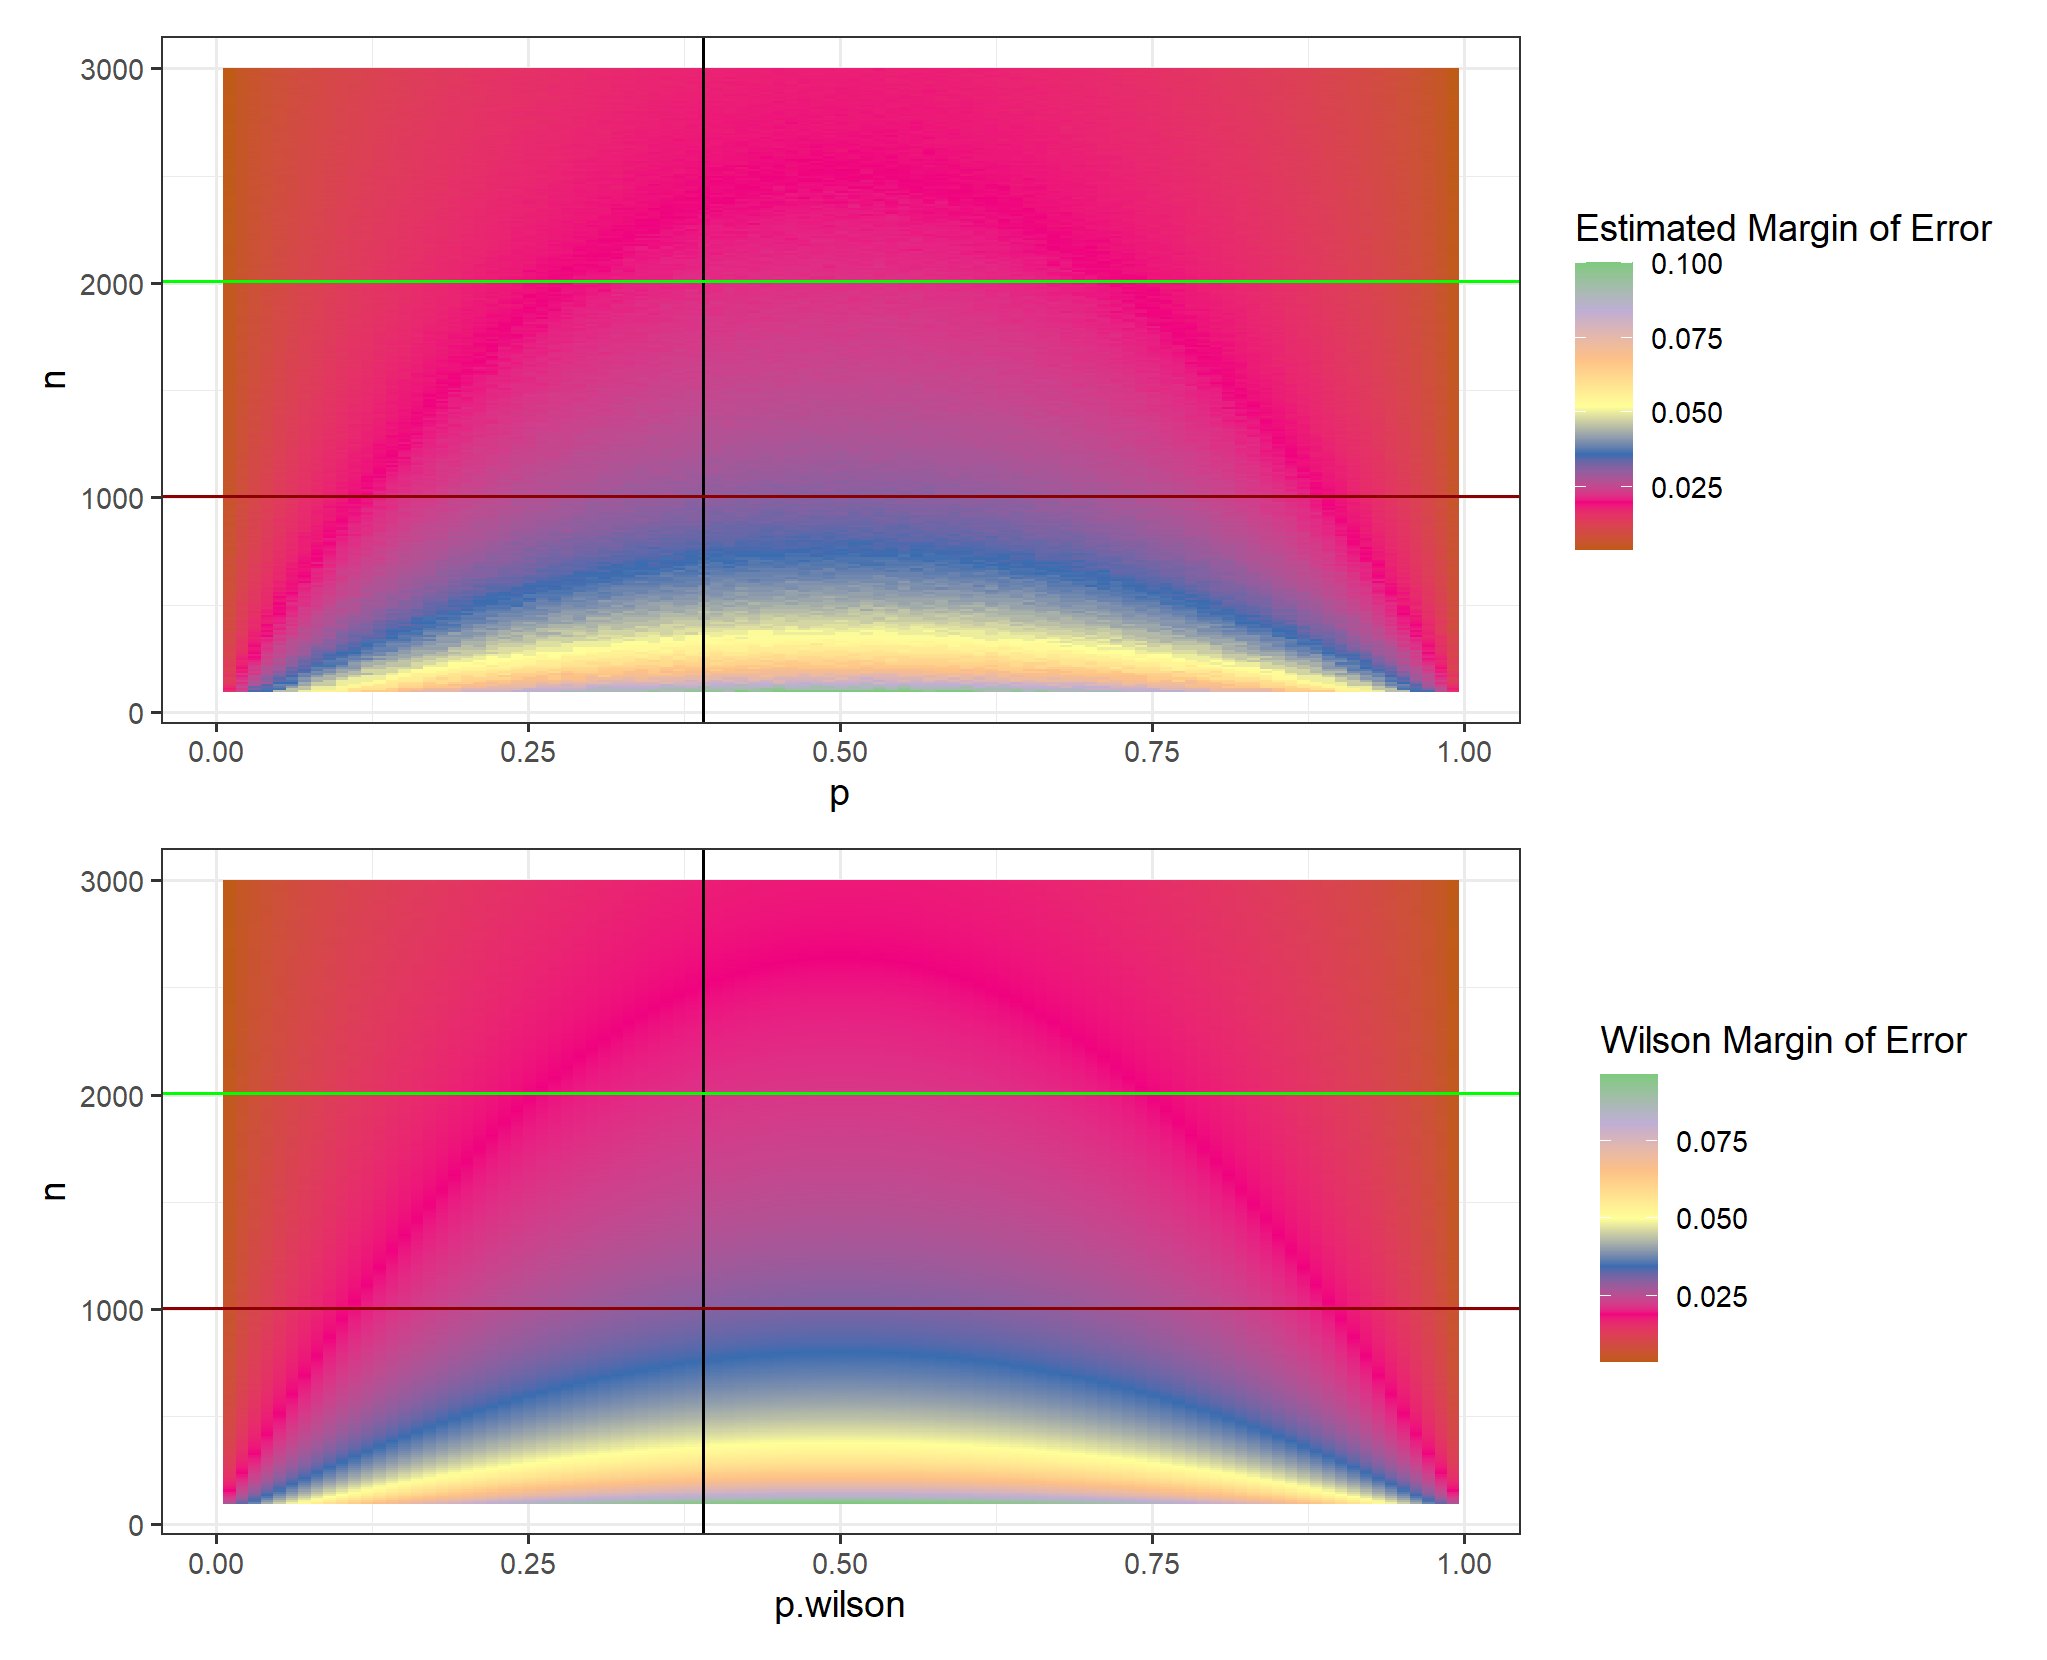
\includegraphics[width = 16cm, height = 14cm]{rasterplots.png}
\captionof{figure}{Plots showing how the estimated MOE varies with $n$ and $p$ (top) and how the Wilson MOE varies with $n$ and $p$.} \label{plot2}
\end{Figure}

\begin{Figure}
\centering
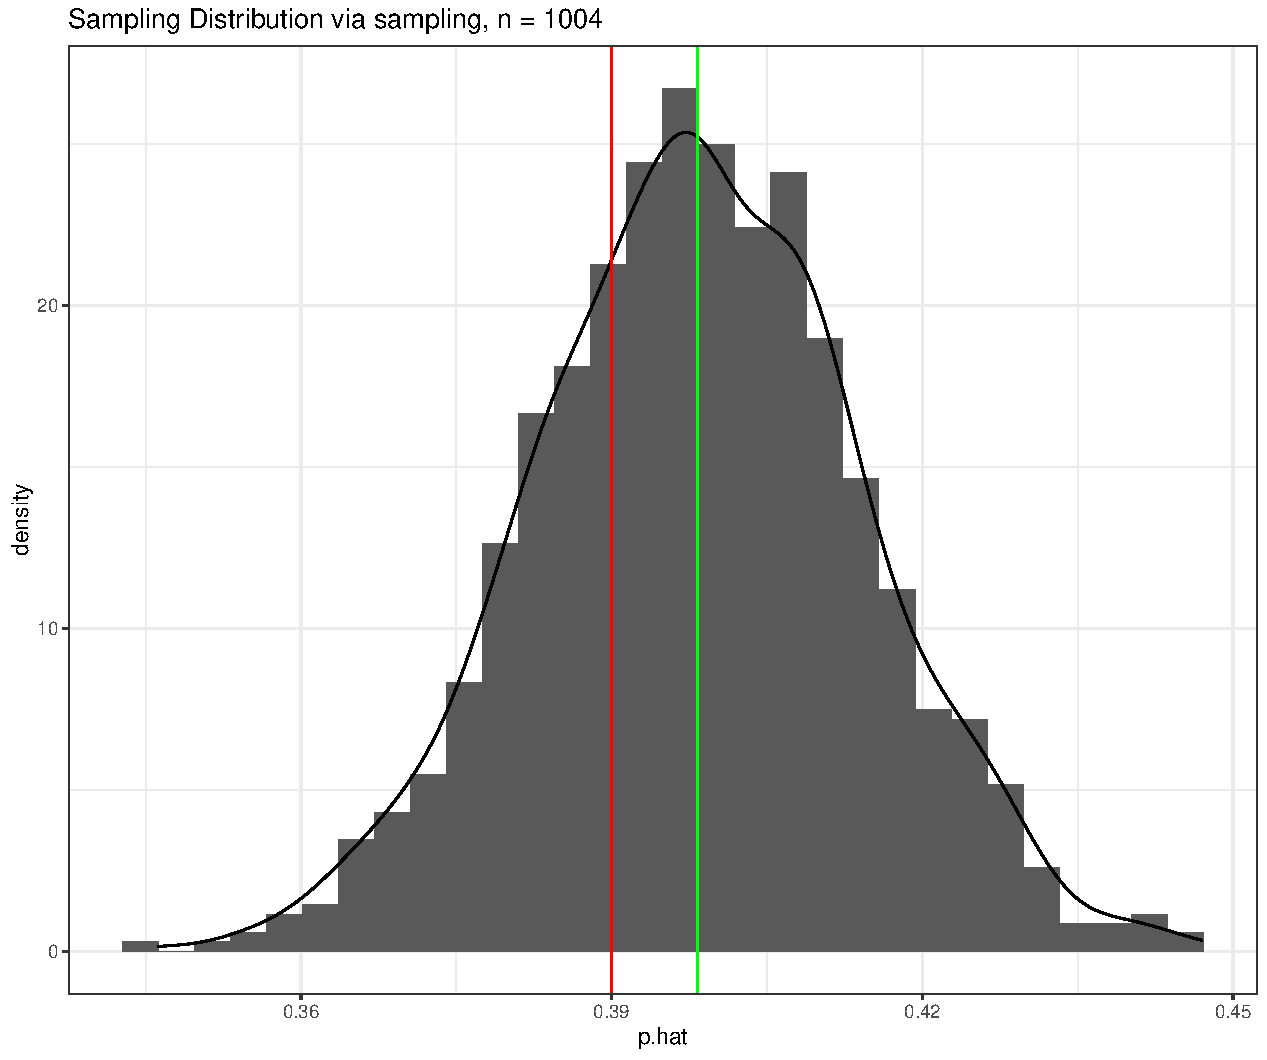
\includegraphics[width = 8cm, height = 6.5cm]{task2histogram.pdf}
\captionof{figure}{Plot showing the sampling distribution for $\hat{p}$ using resampling. For this plot, we conducted $1000$ resamples.} \label{plot3}
\end{Figure}

\end{document}
